
%\begin{center}

      \pagestyle{empty}


\fbox{
  \begin{minipage}[t][22.9cm]{16cm}  %% 24 cm
  \rule{0cm}{5mm}

  \vspace{-.7cm}
  \large  \hfill BNL (2011) \\[-.5cm]

  \vfill
  \vspace{-3cm}
  \title{ 
      \textbf{{\huge ZGOUBI USERS' GUIDE}      
                               }      \\
    }

    \author{ 
      \textbf{Fran\c{c}ois M\'eot } \\
               ~     \\
      { \em Brookhaven National Laboratory   }                       \\
      {\em Collider-Accelerator Department   }      \\
      { \em Upton, NY, 11973 }           
    }

    \maketitle
    \date

    \vfill


      { \Large \hspace{28mm} LHC IP \hspace{45mm} Snake Resonance, RHIC \hfill } 

    \centerline{
      \mbox{
         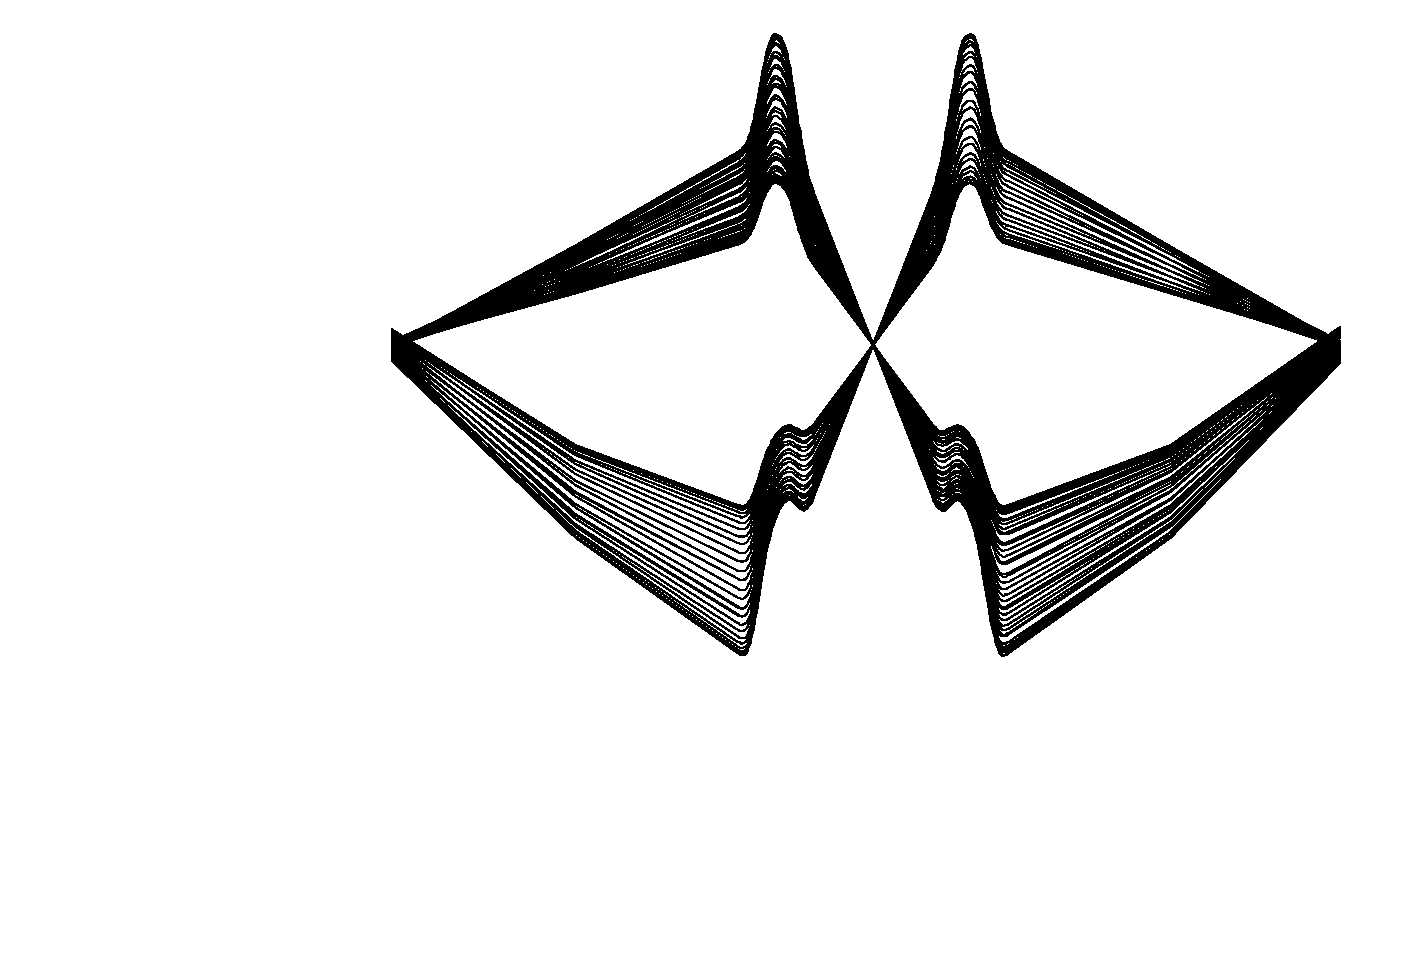
\includegraphics[width=7cm]{FigCover1.ps}
         \hfill
         \includegraphics[width=9cm,height=5cm]{FigCover2New.ps} 
       }
     }


      { \Large \hspace{20mm} Spin flip, AGS \hspace{58mm} DA, NuFact \hfill } 

    \centerline{
      \mbox{
         \hspace{0mm}
         \includegraphics[width=7cm]{FigCover3New.ps}
         \hspace{10mm}
         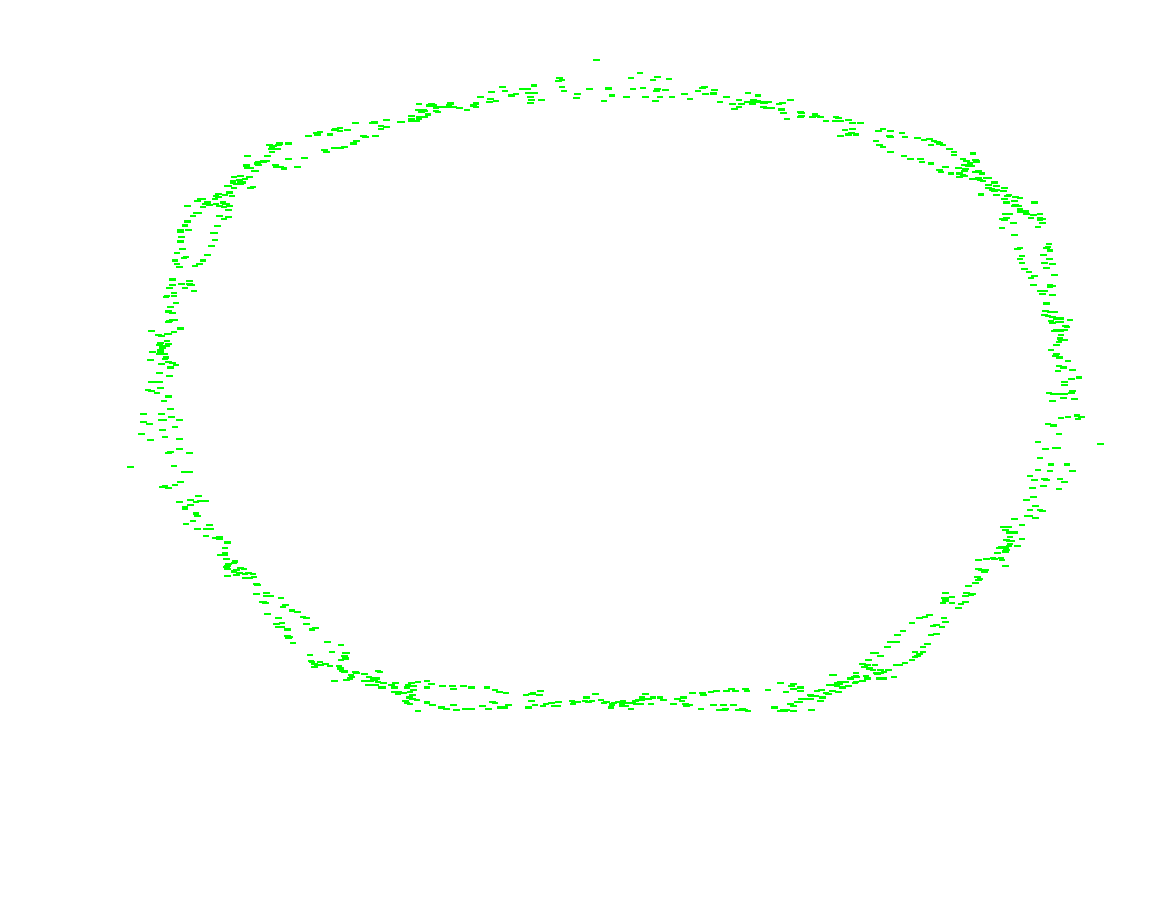
\includegraphics[width=7cm]{FigCover4.ps}
       }
     }

  \end{minipage}
}
%\end{center}


\newpage


~~~~~~~~~~~
  \footnotetext{\Large  {\bf Cover figures} :  \\
  {\it upper left} : collision optics at ATLAS and CMS, \\
  {\it upper right} : polarization upon crossing of 393+$Q_y$ resonance in RHIC,  \\
  {\it lower left} : spin-flipping with partial snakes along AGS cycle,   \\
  {\it lower right} : dynamic aperture in the Neutrino Factory muon decay ring.
   }

